\section{线性模型与可行域}
\label{sec:opt-lp-models}

章首的作坊问题用几句话就能说清，但要交给算法处理，必须先把“产量、获利、原料够不够”翻译成变量、目标和约束。本节先完成这一翻译，并把各种写法统一成一种便于计算的标准表示；随后研究全部可行候选组成的集合长什么样：它的边界由哪些约束决定，从一点出发可以朝哪些方向移动，它什么时候有角点，什么时候根本没有。

\subsection{线性规划的建模与标准型}
\label{sec:opt-lp-modeling}

\paragraph{从资源限制到线性模型}
设两种产品每天的产量分别为$x_1$和$x_2$。每件第一种产品获利$3$，每件第二种产品获利$2$，总获利是$3x_1+2x_2$。第一种原料每天有$4$个单位，两种产品每件分别消耗$2$和$1$个单位，所以产量必须满足$2x_1+x_2\le4$；第二种原料同样有$4$个单位，两种产品每件分别消耗$1$和$2$个单位，于是$x_1+2x_2\le4$。产量不能为负。把这些要求合在一起，得到
\begin{equation}
\label{eq:opt-lp-resource}
  \max_{x_1,x_2}\ 3x_1+2x_2
  \quad\text{s.t.}\quad
  2x_1+x_2\le4,\quad x_1+2x_2\le4,\quad x_1\ge0,\quad x_2\ge0.
\end{equation}
图~\ref{fig:opt-lp-resource-polygon}画出了它的全部可行产量：四条约束各切掉平面的一半，剩下的是以$(0,0)$、$(2,0)$、$(4/3,4/3)$、$(0,2)$为顶点的四边形。绿色直线是获利相同的产量，即目标的等值线$3x_1+2x_2=k$。$k$增大时，等值线沿方向$(3,2)$平行移动；$k=20/3$时它恰好只碰到顶点$(4/3,4/3)$，再增大就离开四边形。于是最大获利是$20/3$，在$x_1=x_2=4/3$处取得。本章后面的每一节都会回到这个例子。

\begin{figure}[!htbp]
  \centering
  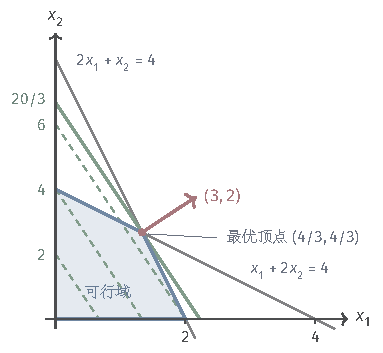
\includegraphics[width=64.904mm]{figures/03-optimization-evolution-and-signals/01-optimization/tikz/c2-resource-polygon/figure.pdf}
  \caption{资源分配例~\eqref{eq:opt-lp-resource}的可行域与目标等值线。浅蓝四边形是满足两条原料约束和非负约束的全部产量，两条灰线是原料恰好用完的边界。绿色虚线是获利为$2$、$4$、$6$的等值线，绿色实线是获利为$20/3$的等值线，纵轴左侧的绿色数字标出各条等值线的获利值；它们都与红色箭头$(3,2)$垂直，沿箭头平移时获利增大。获利$20/3$的等值线只在顶点$(4/3,4/3)$处碰到可行域。}
  \label{fig:opt-lp-resource-polygon}
\end{figure}

这个模型的特点在于目标和每一条约束都是变量的线性函数（可以带常数项）：获利按件数成比例累加，原料消耗也按件数成比例累加，两种产品之间没有相互作用。若生产第一种产品会使第二种产品的单位消耗打折，约束中就会出现$x_1x_2$这样的乘积项，模型不再是线性的。

\begin{definition}[线性规划]
\label{def:opt-lp-linear-program}
在$\mathbb R^n$中，以一个线性函数为目标，在有限个线性等式和非严格线性不等式约束下求最小值或最大值的问题，称为\term{线性规划}（linear programming, LP）。
\end{definition}

定义只允许非严格不等式。若允许$x_1<2$这样的严格不等式，可行域可能不包含它的边界点，最优值可能只能逼近而取不到；非严格不等式定义的可行域是闭集，这为后面最优解的存在性提供了条件。

\paragraph{整数要求不能直接放宽}
若产品只能按整件生产，就要再加上$x_1,x_2\in\mathbb Z$，得到的是\term{整数线性规划}（integer linear programming）。它的可行候选只是图~\ref{fig:opt-lp-resource-polygon}中四边形里的整数点$(0,0)$、$(1,0)$、$(2,0)$、$(0,1)$、$(1,1)$、$(0,2)$，逐个计算获利可知最优的是$(2,0)$，获利$6$。连续模型的解$(4/3,4/3)$不是整数；把它各坐标向下取整得到$(1,1)$，获利只有$5$。所以连续问题的最优解不能直接当作整数问题的解，二者的关系要另外研究，第~\ref{sec:opt-lp-relaxation}节专门处理这个问题。在此之前，本章讨论的都是变量取实数的线性规划。

\paragraph{标准型}
同一个线性规划可以有多种写法：求最大或最小，约束取“$\le$”“$\ge$”或“$=$”，变量有的要求非负，有的可正可负。为了用同一套公式计算，我们约定一种统一的写法。

\begin{definition}[线性规划的标准型]
\label{def:opt-lp-standard-form}
给定$\bm A\in\mathbb R^{m\times n}$、$\bm b\in\mathbb R^m$与$\bm c\in\mathbb R^n$，问题
\begin{equation}
\label{eq:opt-lp-standard}
  \min_{\bm x\in\mathbb R^n}\ \bm c^\top\bm x
  \quad\text{s.t.}\quad
  \bm A\bm x=\bm b,\quad \bm x\ge\bm 0
\end{equation}
称为线性规划的\term{标准型}（standard form），其中$\bm x\ge\bm 0$表示每个分量非负。记它的可行域为$P=\{\bm x\in\mathbb R^n:\bm A\bm x=\bm b,\ \bm x\ge\bm 0\}$。
\end{definition}

本章在讨论线性规划时把变量个数记为$n$、等式约束个数记为$m$，$\bm A$的第$j$列记为$\bm a_j$。下面逐项说明任意线性规划怎样改写成标准型，以及改写前后的解怎样相互恢复。

第一，最大化改为最小化：$\max\bm c^\top\bm x$与$\min(-\bm c)^\top\bm x$有相同的最优解，最优值互为相反数。第二，不等式改为等式：对约束$\bm g^\top\bm x\le h$，引入新变量$s=h-\bm g^\top\bm x$，约束等价于$\bm g^\top\bm x+s=h$且$s\ge0$，$s$称为\term{松弛变量}（slack variable），表示这条约束还剩多少余量；对$\bm g^\top\bm x\ge h$，则减去\term{剩余变量}（surplus variable）$s=\bm g^\top\bm x-h\ge0$。第三，可正可负的\term{自由变量}（free variable）$x_j$写成两个非负变量之差$x_j=x_j^+-x_j^-$。

这些变换保留的是“可行解之间的对应和目标值”，而不一定是一一对应。前两种变换中，新变量由原变量唯一确定，原问题的可行解与新问题的可行解一一对应，目标值不变。第三种变换中，从新问题的可行解总能恢复出$x_j=x_j^+-x_j^-$，目标值不变；但反过来同一个$x_j$有许多表示，例如$x_j=1$既可写成$(x_j^+,x_j^-)=(1,0)$，也可写成$(3,2)$。因此新问题的最优解可能不唯一，而它们都恢复为原问题的同一批最优解。

\begin{example}[资源模型的标准型]
\label{ex:opt-lp-resource-standard}
对模型~\eqref{eq:opt-lp-resource}，把目标改为最小化$-3x_1-2x_2$，并为两条原料约束引入松弛变量$x_3,x_4\ge0$，得到$n=4$、$m=2$的标准型
\[
  \bm A=\begin{pmatrix}2&1&1&0\\1&2&0&1\end{pmatrix},\qquad
  \bm b=\begin{pmatrix}4\\4\end{pmatrix},\qquad
  \bm c=(-3,-2,0,0)^\top.
\]
$x_3=4-2x_1-x_2$与$x_4=4-x_1-2x_2$分别是两种原料的剩余量。原问题的最优点$(4/3,4/3)$对应标准型中的$\bm x=(4/3,4/3,0,0)^\top$，两种原料恰好用完，目标值为$-20/3$。
\end{example}

\subsection{多面体、面与可行方向}
\label{sec:opt-lp-polyhedra}

图~\ref{fig:opt-lp-resource-polygon}中的四边形由四个半平面相交而成。高维情形无法画图，但“由有限个半空间相交”这一描述仍然成立，并足以推出可行域的主要几何性质。第~\ref{chap:optimization}章已经把有限个半空间的交称为多面体；本章统一写成
\[
  Q=\{\bm x\in\mathbb R^d:\bm G\bm x\le\bm h\}
  =\bigcap_{i=1}^k\{\bm x:\bm g_i^\top\bm x\le h_i\},
\]
其中$\bm G\in\mathbb R^{k\times d}$，$\bm h\in\mathbb R^k$，$\bm g_i^\top$是$\bm G$的第$i$行。

每个$\bm g_i\ne\bm 0$时，$\{\bm x:\bm g_i^\top\bm x\le h_i\}$是闭半空间，它的边界$\{\bm x:\bm g_i^\top\bm x=h_i\}$是仿射超平面；等式约束可以写成两个方向相反的不等式，所以有限个等式与不等式共同确定的集合仍是多面体。闭半空间是闭凸集，有限个闭凸集的交仍是闭凸集，所以多面体是闭凸集。标准型的可行域$P$也是多面体：它由$\bm A\bm x\le\bm b$、$-\bm A\bm x\le-\bm b$与$-\bm x\le\bm 0$确定。

\paragraph{活跃约束与面}
在多面体的一点$\bm x$处，有些约束恰好取等号，有些还留有余量。称$\bm g_i^\top\bm x=h_i$的约束为$\bm x$处的\term{活跃约束}（active constraint），记它们的指标集为$I(\bm x)=\{i:\bm g_i^\top\bm x=h_i\}$。对指标集$I\subseteq\{1,\dots,k\}$，令
\[
  F_I=\{\bm x\in Q:\bm g_i^\top\bm x=h_i,\ i\in I\}.
\]
非空的$F_I$称为$Q$的一个\term{面}（face）。取$I=\varnothing$得到$Q$本身；在图~\ref{fig:opt-lp-active-faces}的四边形中，让一条约束取等号得到一条边，让两条相交的约束同时取等号得到一个顶点。不同的指标集可能给出同一个面，例如在第~\ref{sec:opt-lp-degeneracy}节加入第三条过$(2,0)$的约束之后，任选其中两条取等号都得到同一个顶点。

\paragraph{可行方向}
站在可行域中的一点，哪些方向可以走一小步而不离开可行域？这由活跃约束决定。

\begin{definition}[可行方向]
\label{def:opt-lp-feasible-direction}
设$\bm x\in Q$，$\bm d\in\mathbb R^d$。若存在$\varepsilon>0$，使$\bm x+t\bm d\in Q$对全部$t\in[0,\varepsilon]$成立，就称$\bm d$是$Q$在$\bm x$处的\term{可行方向}（feasible direction）。
\end{definition}

\begin{lemma}[多面体的可行方向]
\label{lem:opt-lp-feasible-direction}
设$\bm x\in Q$。$\bm d$是$Q$在$\bm x$处的可行方向，当且仅当$\bm g_i^\top\bm d\le0$对每个$i\in I(\bm x)$成立。
\end{lemma}

\begin{proof}
若某个$i\in I(\bm x)$满足$\bm g_i^\top\bm d>0$，则对任意$t>0$有$\bm g_i^\top(\bm x+t\bm d)=h_i+t\bm g_i^\top\bm d>h_i$，所以$\bm d$不是可行方向。反过来，设全部活跃约束都满足$\bm g_i^\top\bm d\le0$。对活跃约束，$\bm g_i^\top(\bm x+t\bm d)\le h_i$对所有$t\ge0$成立。不活跃的约束有余量$h_i-\bm g_i^\top\bm x>0$；若$\bm g_i^\top\bm d\le0$，它对所有$t\ge0$都成立，否则只要$t\le(h_i-\bm g_i^\top\bm x)/\bm g_i^\top\bm d$就仍成立。不活跃约束只有有限条，取这些正上界中的最小值作为$\varepsilon$（没有正上界时取$\varepsilon=1$）即可。
\end{proof}

引理把“能否移动”变成了只看活跃约束的有限个线性不等式。图~\ref{fig:opt-lp-active-faces}画出了三种典型位置。内部点没有活跃约束，任何方向都可以走；边上的点只有一条活跃约束，例如在边$2x_1+x_2=4$上，可行方向是满足$2d_1+d_2\le0$的半平面；在顶点$(4/3,4/3)$处两条约束同时活跃，可行方向是同时满足$2d_1+d_2\le0$与$d_1+2d_2\le0$的锥，它由$(1,-2)$和$(-2,1)$两个边方向张成，正好指向可行域内部。活跃约束越多，能走的方向越少。

\begin{figure}[!htbp]
  \centering
  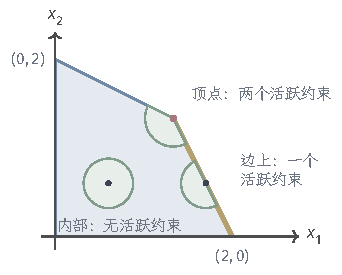
\includegraphics[width=57.993mm]{figures/03-optimization-evolution-and-signals/01-optimization/tikz/c2-active-faces/figure.pdf}
  \caption{活跃约束与可行方向。在资源分配例的可行域中，绿色区域表示从黑点或红点出发可以走一小步的方向：内部点处是整个圆盘，边上的点处是半个圆盘，顶点$(4/3,4/3)$处是两条边方向张成的锥。黄色粗线是约束$2x_1+x_2\le4$取等号得到的面，即一条边。}
  \label{fig:opt-lp-active-faces}
\end{figure}

\paragraph{极点}
顶点在图中一眼就能认出，但高维时需要一个不依赖图形的定义。观察图~\ref{fig:opt-lp-active-faces}：内部点和边上的点都位于某条可行线段的中间，顶点却不是任何两个不同可行点连线的中间点。

\begin{definition}[极点]
\label{def:opt-lp-extreme-point}
设$C$是凸集，$\bm x\in C$。若$\bm x=\lambda\bm u+(1-\lambda)\bm v$、$\bm u,\bm v\in C$、$\lambda\in(0,1)$总推出$\bm u=\bm v=\bm x$，就称$\bm x$是$C$的\term{极点}（extreme point）。
\end{definition}

在二维例子中，极点恰好是两条线性无关的约束同时取等号的点。下一节将在标准型中证明相应的一般结论：极点就是可以由一个线性方程组解出的“基本可行解”。

\paragraph{空集、有界与无界}
多面体可以有几种很不相同的形状，图~\ref{fig:opt-lp-polyhedron-cases}列出了与线性规划有关的几种。约束彼此矛盾时多面体是空集，例如在第一象限中同时要求$x_1+x_2\le1$与$x_1+x_2\ge2$。多面体也可以无界。若$Q$非空，且方向$\bm d$满足$\bm G\bm d\le\bm 0$，则对任意$\bm x\in Q$和$t\ge0$都有$\bm G(\bm x+t\bm d)\le\bm h$，即沿$\bm d$可以一直走下去而不离开$Q$；这样的$\bm d$称为$Q$的\term{回收方向}（recession direction）。

可行域无界并不意味着目标无下界。图~\ref{fig:opt-lp-polyhedron-cases}(b)与(c)用的是同一个无界区域$\{x_1\ge0,\ x_2\ge0,\ x_1+x_2\ge1\}$。最小化$x_1+2x_2$时，所有回收方向$\bm d\ge\bm 0$都使目标不减，最小值$1$在$(1,0)$处达到；最小化$x_2-x_1$时，沿回收方向$\bm d=(1,0)$走$t$步，目标减少$t$，所以没有下界。决定目标有无下界的是目标沿回收方向的变化，而不是可行域是否有界。反过来，若可行域非空且有界，它是$\mathbb R^d$中的有界闭集，连续的线性目标一定能取到最小值。

\begin{figure*}[!htbp]
  \centering
  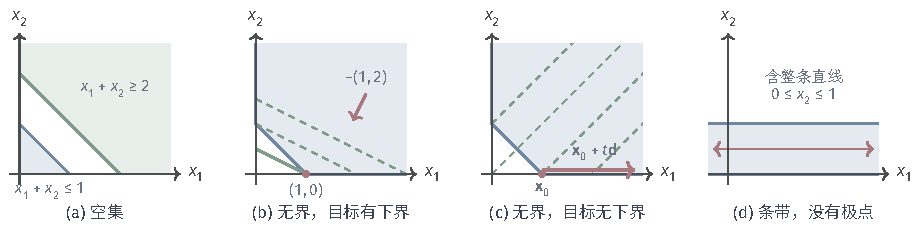
\includegraphics[width=156.496mm]{figures/03-optimization-evolution-and-signals/01-optimization/tikz/c2-polyhedron-cases/figure.pdf}
  \caption{几种多面体。(a) 第一象限中$x_1+x_2\le1$的部分（蓝）与$x_1+x_2\ge2$的部分（绿）不相交，多面体为空集。(b) 无界区域$\{x_1,x_2\ge0,\ x_1+x_2\ge1\}$上最小化$x_1+2x_2$，绿色线为等值线，红色箭头是目标下降的方向，最小值$1$在$(1,0)$处达到。(c) 同一区域上最小化$x_2-x_1$，从$\bm x_0=(1,0)$沿$\bm d=(1,0)$前进，目标无限下降。(d) 条带$0\le x_2\le1$（$x_1$不受限制）包含整条水平直线，没有极点。}
  \label{fig:opt-lp-polyhedron-cases}
\end{figure*}

\paragraph{直线、条带与最优面}
多面体还可能根本没有极点。图~\ref{fig:opt-lp-polyhedron-cases}(d)的条带$\{(x_1,x_2):0\le x_2\le1\}$对每个点都包含一整条水平直线：任何点都是左右两个可行点的中点，所以没有极点。直线$\{(x_1,0):x_1\in\mathbb R\}$本身也是多面体，同样没有极点。在这样的区域上最小化$x_2$，最小值$0$在整条直线上取得，却没有一个“角点”可以代表它。

标准型的可行域$P$不会出现这种情况。若$\bm x+t\bm d\in P$对全部实数$t$成立，则每个坐标$x_j+td_j$对正负两个方向的$t$都非负，只能有$d_j=0$；所以$P$不包含任何直线。下一节正是利用这一点证明：非空的$P$一定有极点，并且有限的最优值一定能在某个极点处取得。这也是我们选择标准型作为计算对象的一个理由。

最后，最优解不一定唯一。若目标的等值线恰好与可行域的一条边平行，在等值线平移到最后时，它接触的是整条边，边上每一点都是最优解，例如图~\ref{fig:opt-lp-optimal-face}(b)。全部最优解组成的集合$\{\bm x\in Q:\bm c^\top\bm x=f^\star\}$称为\term{最优面}（optimal face），其中$f^\star$是最优值；它是凸集；对标准型，第~\ref{sec:opt-lp-strong-duality}节会说明它确实是可行域的一个面。从图形上看到等值线接触到可行域，只能说明找到了最优值，不能据此断言最优解唯一。
